\documentclass[tikz,border=5pt]{standalone}
\usepackage{ctex,amsmath}
\usetikzlibrary{arrows.meta,calc,angles,quotes}
\tikzset{>=Latex,current/.style={orange!85!black,thick,->},
 point/.style={blue!65!black},guide/.style={gray,dashed},
 volt/.style={blue!60!black,thin}}
\begin{document}
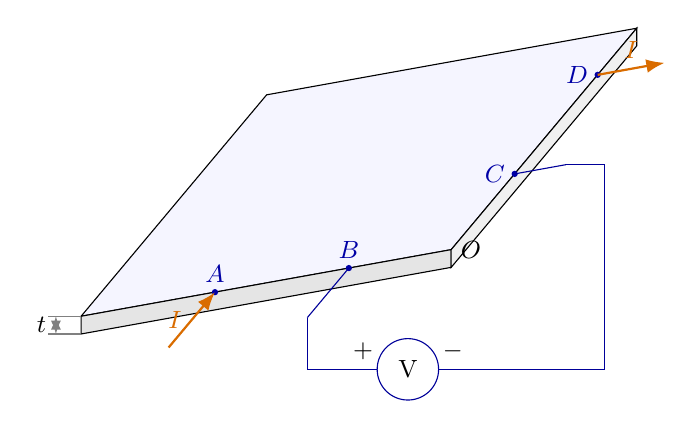
\begin{tikzpicture}[font=\small,x={(-1cm,-.18cm)},y={(.62cm,.74cm)},z={(0cm,.5cm)}]
\coordinate(O)at(0,0,0);\coordinate(A)at(3,0,0);\coordinate(B)at(1.3,0,0);
\coordinate(C)at(0,1.3,0);\coordinate(D)at(0,3,0);
\filldraw[fill=blue!4,draw=black](0,0,0)--(4.7,0,0)--(4.7,3.8,0)--(0,3.8,0)--cycle;
\filldraw[fill=gray!20](0,0,0)--(4.7,0,0)--(4.7,0,-.45)--(0,0,-.45)--cycle;
\filldraw[fill=gray!12](0,0,0)--(0,3.8,0)--(0,3.8,-.45)--(0,0,-.45)--cycle;
\foreach \pt/\pos in {A/above,B/above,C/left,D/left}{
 \fill[point](\pt)circle[radius=.04cm]node[\pos]{$\pt$};}
\node[right]at(O){$O$};
\draw[current](3,-.95,0)--(A)node[midway,left]{$I$};
\draw[current](D)--(-.85,3,0)node[midway,above]{$I$};
\draw[volt](B)--(1.3,-.85,0);
\draw[volt](C)--(-.65,1.3,0);
\begin{scope}[x={(1cm,0cm)},y={(0cm,1cm)},z={(0cm,0cm)}]
\draw[volt](-1.827,-.863)--(-1.827,-1.52)--(-.94,-1.52);
\draw[volt](1.456,1.079)--(1.95,1.079)--(1.95,-1.52)--(-.16,-1.52);
\draw[volt](-.55,-1.52)circle[radius=.39cm];
\node at(-.55,-1.52){V};\node[above]at(-1.12,-1.52){$+$};\node[above]at(.02,-1.52){$-$};
\draw[<->,gray](-5.02,-.846)--(-5.02,-1.071)node[midway,left,text=black]{$t$};
\draw[gray](-4.7,-.846)--(-5.12,-.846);\draw[gray](-4.7,-1.071)--(-5.12,-1.071);
\end{scope}
\end{tikzpicture}
\begin{tikzpicture}[font=\small,scale=1.15]
\fill[blue!4](0,0)rectangle(2.4,2.4);
\draw[->,gray](-2.2,0)--(2.5,0)node[right]{$x$};
\draw[->,gray](0,-2.2)--(0,2.5)node[above]{$y$};
\draw[very thick](0,2.35)--(0,0)--(2.35,0);
\draw(.2,0)--(.2,.2)--(0,.2);
\coordinate(A)at(1.65,0);\coordinate(As)at(-1.65,0);
\coordinate(D)at(0,1.65);\coordinate(Ds)at(0,-1.65);
\coordinate(B)at(.74,0);\coordinate(C)at(0,.74);
\fill[orange!85!black](A)circle[radius=.04]node[below]{$A:+2I$};
\fill[orange!85!black](As)circle[radius=.04]node[below]{$A^*:+2I$};
\fill[blue!65!black](D)circle[radius=.04]node[left]{$D:-2I$};
\fill[blue!65!black](Ds)circle[radius=.04]node[left]{$D^*:-2I$};
\fill[black](B)circle[radius=.028]node[below]{$B$};
\fill[black](C)circle[radius=.028]node[left]{$C$};
\draw[guide](B)--(D);\draw[guide](B)--(Ds);
\node[fill=white,inner sep=1.5pt,rotate=-66]at(.44,1.0){$l\sqrt{1+\lambda^2}$};
\draw[<->,gray](.74,-.48)--(1.65,-.48)node[midway,below,text=black]{$(1-\lambda)l$};
\node[above right]at(0,0){$O$};
\node[align=center]at(1.38,2.1){真实板区域};
\node[below]at(0,-2.6){全平面等效源、汇；真实接触电流仍为 $I$};
\end{tikzpicture}
\begin{tikzpicture}[font=\small]
\begin{scope}
\fill[blue!4](-2.3,0)rectangle(2.3,2.05);
\draw[thick](-2.3,0)--(2.3,0);
\coordinate(A)at(0,0);
\fill[orange!85!black](A)circle[radius=.04]node[below right]{$A$};
\draw[current](0,-.7)--(A)node[midway,left]{$I$};
\draw[blue!65!black,thick](1.35,0)arc[start angle=0,end angle=180,radius=1.35];
\draw[guide](A)--({1.35*cos(40)},{1.35*sin(40)})node[midway,below right]{$\rho$};
\foreach \angle in {30,70,110,150}{
 \draw[current]({.82*cos(\angle)},{.82*sin(\angle)})--({1.63*cos(\angle)},{1.63*sin(\angle)});
}
\node at(0,2.4){边缘接触};
\node[below]at(0,-1){截流面积 $\pi\rho t$};
\end{scope}
\begin{scope}[xshift=6.2cm]
\fill[blue!4](-2.3,-2.05)rectangle(2.3,2.05);
\fill[orange!85!black](0,0)circle[radius=.04]node[below right]{$A_0$};
\draw[blue!65!black,thick](0,0)circle[radius=1.35];
\draw[guide](0,0)--({1.35*cos(40)},{1.35*sin(40)})node[midway,below right]{$\rho$};
\foreach \angle in {30,70,110,150,210,250,290,330}{
 \draw[current]({.82*cos(\angle)},{.82*sin(\angle)})--({1.63*cos(\angle)},{1.63*sin(\angle)});
}
\node at(0,2.4){全平面等效接触};
\node[below]at(0,-2.3){总电流 $2I$，截流面积 $2\pi\rho t$};
\end{scope}
\end{tikzpicture}
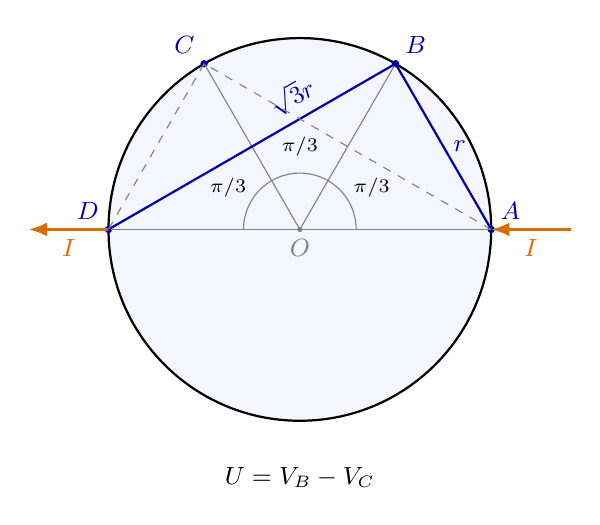
\begin{tikzpicture}[font=\small,scale=1.35]
\filldraw[fill=blue!4,thick](0,0)circle[radius=1.8];
\coordinate(O)at(0,0);\coordinate(A)at(1.8,0);\coordinate(D)at(-1.8,0);
\coordinate(B)at(.9,1.55885);\coordinate(C)at(-.9,1.55885);
\fill[gray](O)circle[radius=.025]node[below]{$O$};
\foreach \pt/\pos in {A/above right,B/above right,C/above left,D/above left}{
 \fill[point](\pt)circle[radius=.035]node[\pos]{$\pt$};}
\foreach \pt in {A,B,C,D}\draw[gray,thin](O)--(\pt);
\foreach \start in {0,60,120}{
 \draw[gray]({.53*cos(\start)},{.53*sin(\start)})arc[start angle=\start,end angle=\start+60,radius=.53];
 \node[font=\scriptsize]at({.78*cos(\start+30)},{.78*sin(\start+30)}){$\pi/3$};
}
\draw[blue!65!black,thick](A)--(B)node[midway,right]{$r$};
\draw[blue!65!black,thick](B)--(D)node[pos=.32,above,sloped]{$\sqrt3r$};
\draw[guide](A)--(C);\draw[guide](C)--(D);
\draw[current](2.55,0)--(A)node[midway,below]{$I$};
\draw[current](D)--(-2.55,0)node[midway,below]{$I$};
\node[below]at(0,-2.15){$U=V_B-V_C$};
\end{tikzpicture}
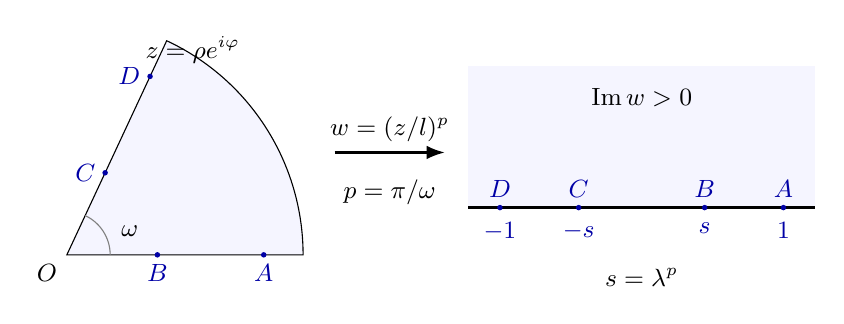
\begin{tikzpicture}[font=\small]
\begin{scope}
\filldraw[fill=blue!4](0,0)--(3,0)arc[start angle=0,end angle=65,radius=3]--cycle;
\coordinate(O)at(0,0);
\foreach \rr/\name/\angle/\pos in {2.5/A/0/below,1.15/B/0/below,1.15/C/65/left,2.5/D/65/left}{
 \fill[point]({\rr*cos(\angle)},{\rr*sin(\angle)})circle[radius=.035]node[\pos]{$\name$};
}
\draw[gray](.55,0)arc[start angle=0,end angle=65,radius=.55];
\node at(.8,.3){$\omega$};\node[below left]at(O){$O$};
\node at(1.6,2.6){$z=\rho e^{i\varphi}$};
\end{scope}
\draw[->,thick](3.4,1.3)--(4.8,1.3)node[midway,above]{$w=(z/l)^p$};
\node at(4.1,.8){$p=\pi/\omega$};
\begin{scope}[xshift=7.3cm,yshift=.6cm]
\fill[blue!4](-2.2,0)rectangle(2.2,1.8);
\draw[thick](-2.2,0)--(2.2,0);
\foreach \xx/\name/\label in {-1.8/D/-1,-.8/C/-s,.8/B/s,1.8/A/1}{
 \fill[point](\xx,0)circle[radius=.035]node[above]{$\name$}node[below,yshift=-2pt]{$\label$};
}
\node[below]at(0,-.65){$s=\lambda^p$};
\node at(0,1.4){$\operatorname{Im}w>0$};
\end{scope}
\end{tikzpicture}
\end{document}
